% --------------------------------------------------------------
% This is all preamble stuff that you don't have to worry about.
% Head down to where it says "Start here"
% --------------------------------------------------------------

\documentclass[12pt]{article}

\usepackage[margin=1in]{geometry} 
\usepackage{amsmath,amsthm,amssymb}
\usepackage{graphicx}

\newcommand{\N}{\mathbb{N}}
\newcommand{\Z}{\mathbb{Z}}

\newenvironment{theorem}[2][Theorem]{\begin{trivlist}
		\item[\hskip \labelsep {\bfseries #1}\hskip \labelsep {\bfseries #2.}]}{\end{trivlist}}
\newenvironment{lemma}[2][Lemma]{\begin{trivlist}
		\item[\hskip \labelsep {\bfseries #1}\hskip \labelsep {\bfseries #2.}]}{\end{trivlist}}
\newenvironment{exercise}[2][Exercise]{\begin{trivlist}
		\item[\hskip \labelsep {\bfseries #1}\hskip \labelsep {\bfseries #2.}]}{\end{trivlist}}
\newenvironment{reflection}[2][Reflection]{\begin{trivlist}
		\item[\hskip \labelsep {\bfseries #1}\hskip \labelsep {\bfseries #2.}]}{\end{trivlist}}
\newenvironment{proposition}[2][Proposition]{\begin{trivlist}
		\item[\hskip \labelsep {\bfseries #1}\hskip \labelsep {\bfseries #2.}]}{\end{trivlist}}
\newenvironment{corollary}[2][Corollary]{\begin{trivlist}
		\item[\hskip \labelsep {\bfseries #1}\hskip \labelsep {\bfseries #2.}]}{\end{trivlist}}

\begin{document}
	
	% --------------------------------------------------------------
	%                         Start here
	% --------------------------------------------------------------
	
	%\renewcommand{\qedsymbol}{\filledbox}
	
	
	\title{Computational Topology \\ Homework 2}
	\author{%replace with your name
		Bernarda Petek} %if necessary, replace with your course title
	
	\date{December 4, 2022}
	\maketitle
	
	\section{Theoretical problems}
	\subsection{Triangulations}
	$S$ is a set of $n$ points in the plane, $n \in \mathbb{N}$. \\
	
	
	 \textbf{(a)} In this exercise I will prove that for all $n \in \mathbb{N}$ there are at most $2^{\frac{n\cdot (n-1)}{2}}$ triangulations by using graph theory and combinatorics. Every triangulation can be seen as a graph where points in $S$ are vertices. We know that in complete graph where every point is connected to every other point there are $\frac{n\cdot (n-1)}{2}$ edges. So edges of every triangulation are a subset of edges in complete graph on the same vertices. So for every edge we can say that it either belongs to the triangulation or not. To get all possible triangulations we can look at all possible combinations of edges, which is a combinatorial problem. To get all combinations we have two options for every edge - either it belongs in the triangulation or it does not. Because we have at most $\frac{n\cdot (n-1)}{2}$ edges there are at most  $2^{\frac{n\cdot (n-1)}{2}}$ different combinations and those are also all possible triangulations. Ofcourse not all of them are valid.
	 
	 \textbf{(b)} In the second part of the exercise I will construct a set $S$ of $n$ points for every $n \in \mathbb{N}, n \geq 3$ such that all possible triangulations of $S$ have a point of degree $n-1$. Such set $S$ consists of $n-1$ collinear points and one point that is collinear to at most one of them. Because all except one point are collinear no three connected points can form a triangle that is not deformed. The only way triangles can be formed are by connecting the point that is not collinear to all other points with all the other points that are collinear and by connecting every one of the collinear points by its neighbour. The point that is not collinear to all other points is exactly the point we are looking for. It has the degree $n-1$ because it is connected to all the other points. For $n=5$ I drew an example which can be seen on Figure \ref{fig:1}.
	 
	 \begin{figure}
	 	\centering
	 	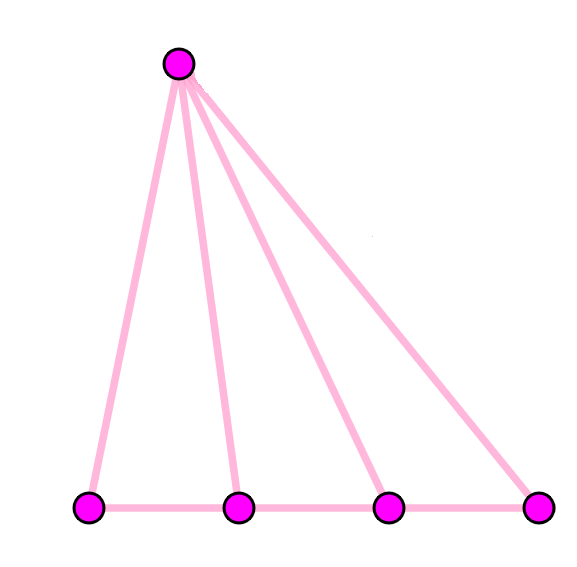
\includegraphics[scale=0.20] {graf1}
	 	\caption{\label{fig:1} Example for $n=5$ for (b) of Exercise 1. }
	 \end{figure}
	 
	 \textbf{(c)} In the last part of the first exercise I will prove that any triangulation $T$ of $S$ has a point of degree $5$ or less by using proof by contradiction. Let's assume that there exists a triangulation $T$ of $S$ where every point has a degree $6$ or more. There are at least $\frac{6n}{2}$ edges in such triangulation because the triangulation has $n$ points, every point has at least 6 edges so together $6n$ edges but the whole number is divided by $2$ so that we don't count the same edges twice. Consequently there are at least $\frac{6n}{2} = 3n$ edges in triangulation $T$. And that is a contraditicon with the fact that any triangulation $T$ of $S$ has at most $3n-3$ edges. End of proof.
	
	\subsection{Vietoris-Rips Complex and Čech Complex}
	Let's label the points from $S$ as $A=(0,0)$, $B=(2,0)$, $C=(1,0.5)$,$D=(1,1.5)$. \\
	
	\begin{figure}
		\centering
		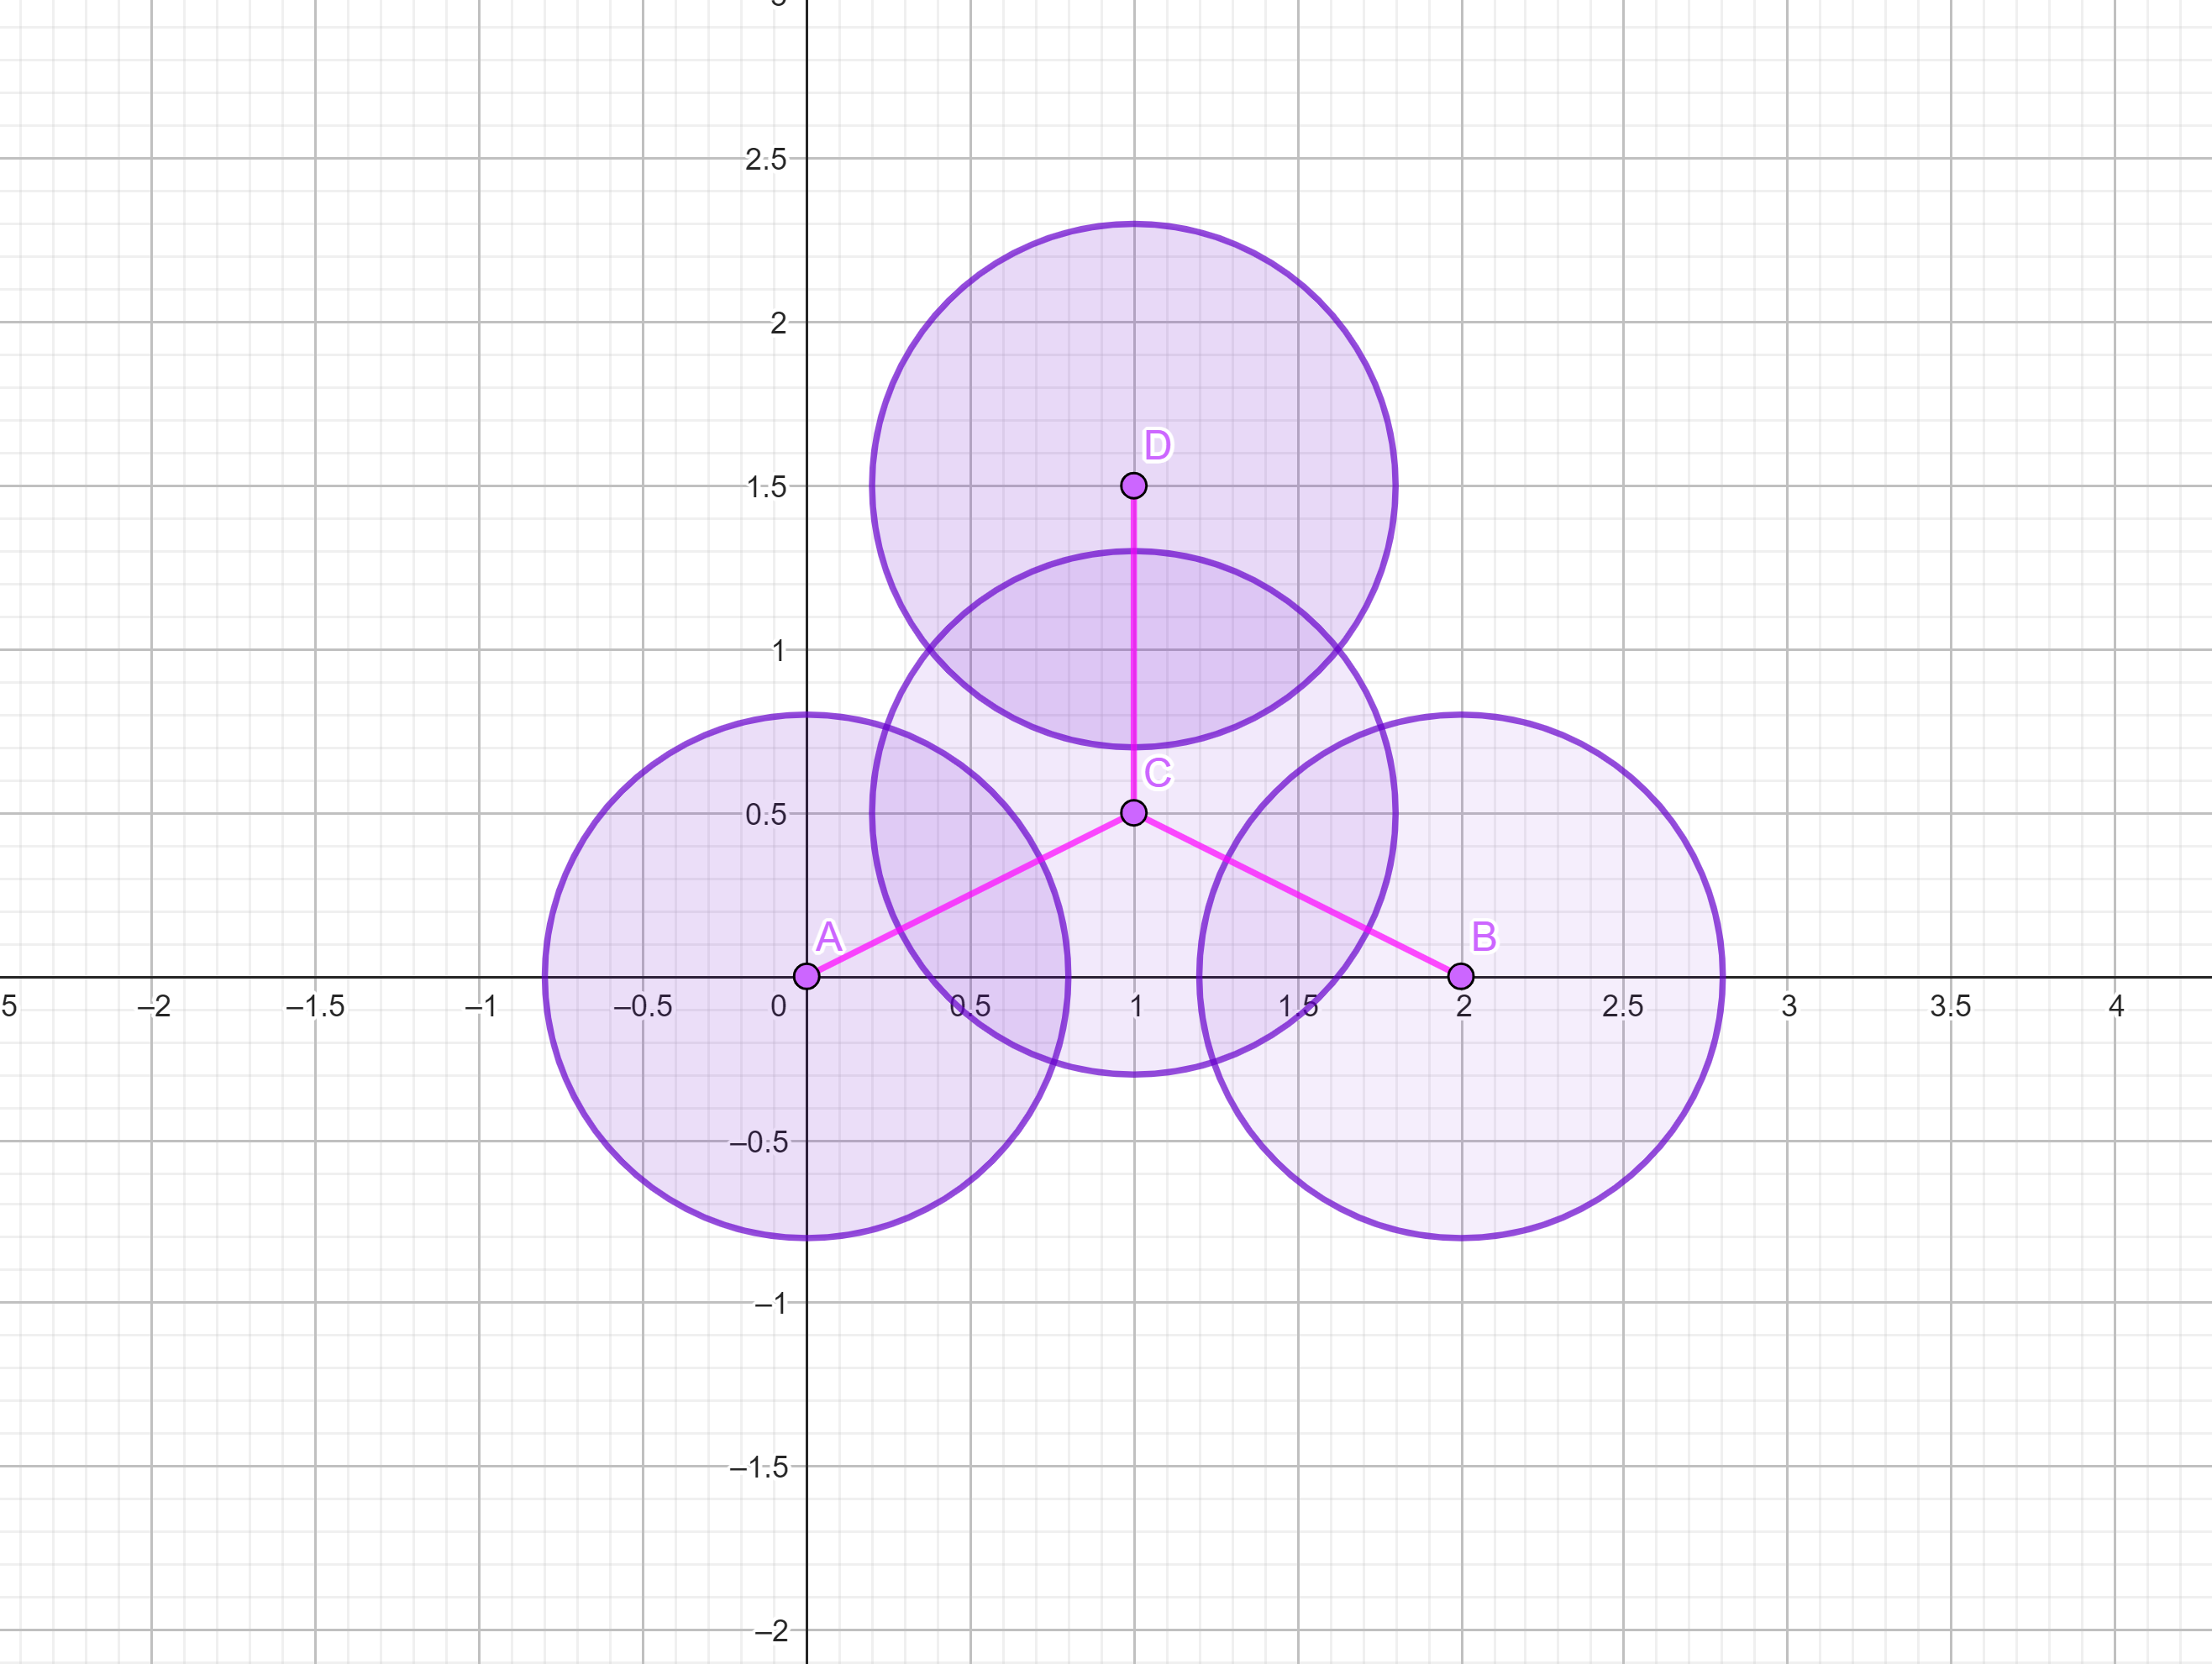
\includegraphics[scale=0.20] {graf3}
		\caption{\label{fig:1} Closed balls around the points and skeleton of $VR_{1.6}(S)$ . }
	\end{figure}
	
	\textbf{(a)}  To build a Vietoris-Rips complex $VR_{2\cdot \epsilon}(S)$ and Čech complex Č$_{\epsilon}(S)$ for $\epsilon = 0.8$ I drew four closed balls with radius 0.8 with origin points $A,B,C,D$. This can be seen on Figure 2. I did that because in the Vietoris-Rips complex $VR_{2\cdot \epsilon}(S)$ two vertices are connected by an edge if and only if the distance between them is at most $2\cdot \epsilon = 1.6$. The graph I obtained is the 1-skeleton of $VR_{1.6}(S)$. From the graph I can list all the simplices (because there are no other complete subgraphs): 
	 $$VR_{1.6}(S) = \{A,B,C,D,CA,CB,CD\}$$
	 
	 There are no simplices of dimension higher than 1 so dim$VR_{1.6}(S) = 1$. The Euler characteristic is $\chi = 4-3=1$. Because we know that the skeleton of Č$_{0.8}(S)$ is the same as the skeleton of $VR_{1.6}(S)$ which is actually $VR_{1.6}(S)$ itself and also because we know that $C_{0.8}(S) \subseteq VR_{1.6}(S)$ we can also see that:
	 
	  $$\check{C}_{0.8}(S) = \{A,B,C,D,CA,CB,CD\}$$ 
	  
	  and consequently dimČ$_{1.6}(S) = 1$ and its Euler characteristic is  $\chi = 4-3=1$.
	  
	  \textbf{(b)} To build a Vietoris-Rips complex $VR_{2\cdot \epsilon}(S)$ and Čech complex Č$_{\epsilon}(S)$ for $\epsilon = 1$ I did the exact same thing as before, only this time the closed balls had radius 1, which can be seen on Figure 3. We can see from the drawing the skeleton of the $VR_{2}(S)$ which is the subset of the $VR_{2}(S)$. We can also see that the skeleton contains three $K_3$ which means that $VR_{2}(S)$ contains three 2-simplices which are: $ABC$, $BCD$ and $ACD$. The skeleton also contains one $K_4$ which means that $VR_{2}(S)$ contains one 3-simplex: $ABCD$. So:
	  $$VR_{2}(S) = \{A,B,C,D,CA,CB,CD,AB,BD,DA,ABC,BCD,ACD,ABCD\}$$
	  
	 There are no simplices of dimension higher than 3 so dim$VR_{2}(S) = 3$. The Euler characteristic is $\chi = 4-6+3-1=0$. We know that $C_{1}(S) \subseteq VR_{2}(S)$ and we know that their skeletons are the same. That means that we only have to check the intersections between balls in 2- and 3- dimensional simplices from $VR_{2}(S)$ which are: $ABC,BCD,ACD,ABCD$. We can see that intersection of the circles centered at $A,B,C$ is not empty so that means that $ABC$ is a 2-simplex in $C_{1}(S)$. Same goes for $BCD, ACD$. However, intersection of the circles centered at $A,B,C,D$ is empty so $ABCD$ is not a 3-simplex in $C_{1}(S)$. That means: 
	 
	  $$\check{C}_{1}(S) = \{A,B,C,D,CA,CB,CD,AB,BD,DA,ABC,BCD,ACD\}$$
	  
	  Subsequently. dimČ$_{1}(S) = 2$ and its Euler characteristic is $\chi = 4-6+3=1$. 
	  
	  	\begin{figure}
	  	\centering
	  	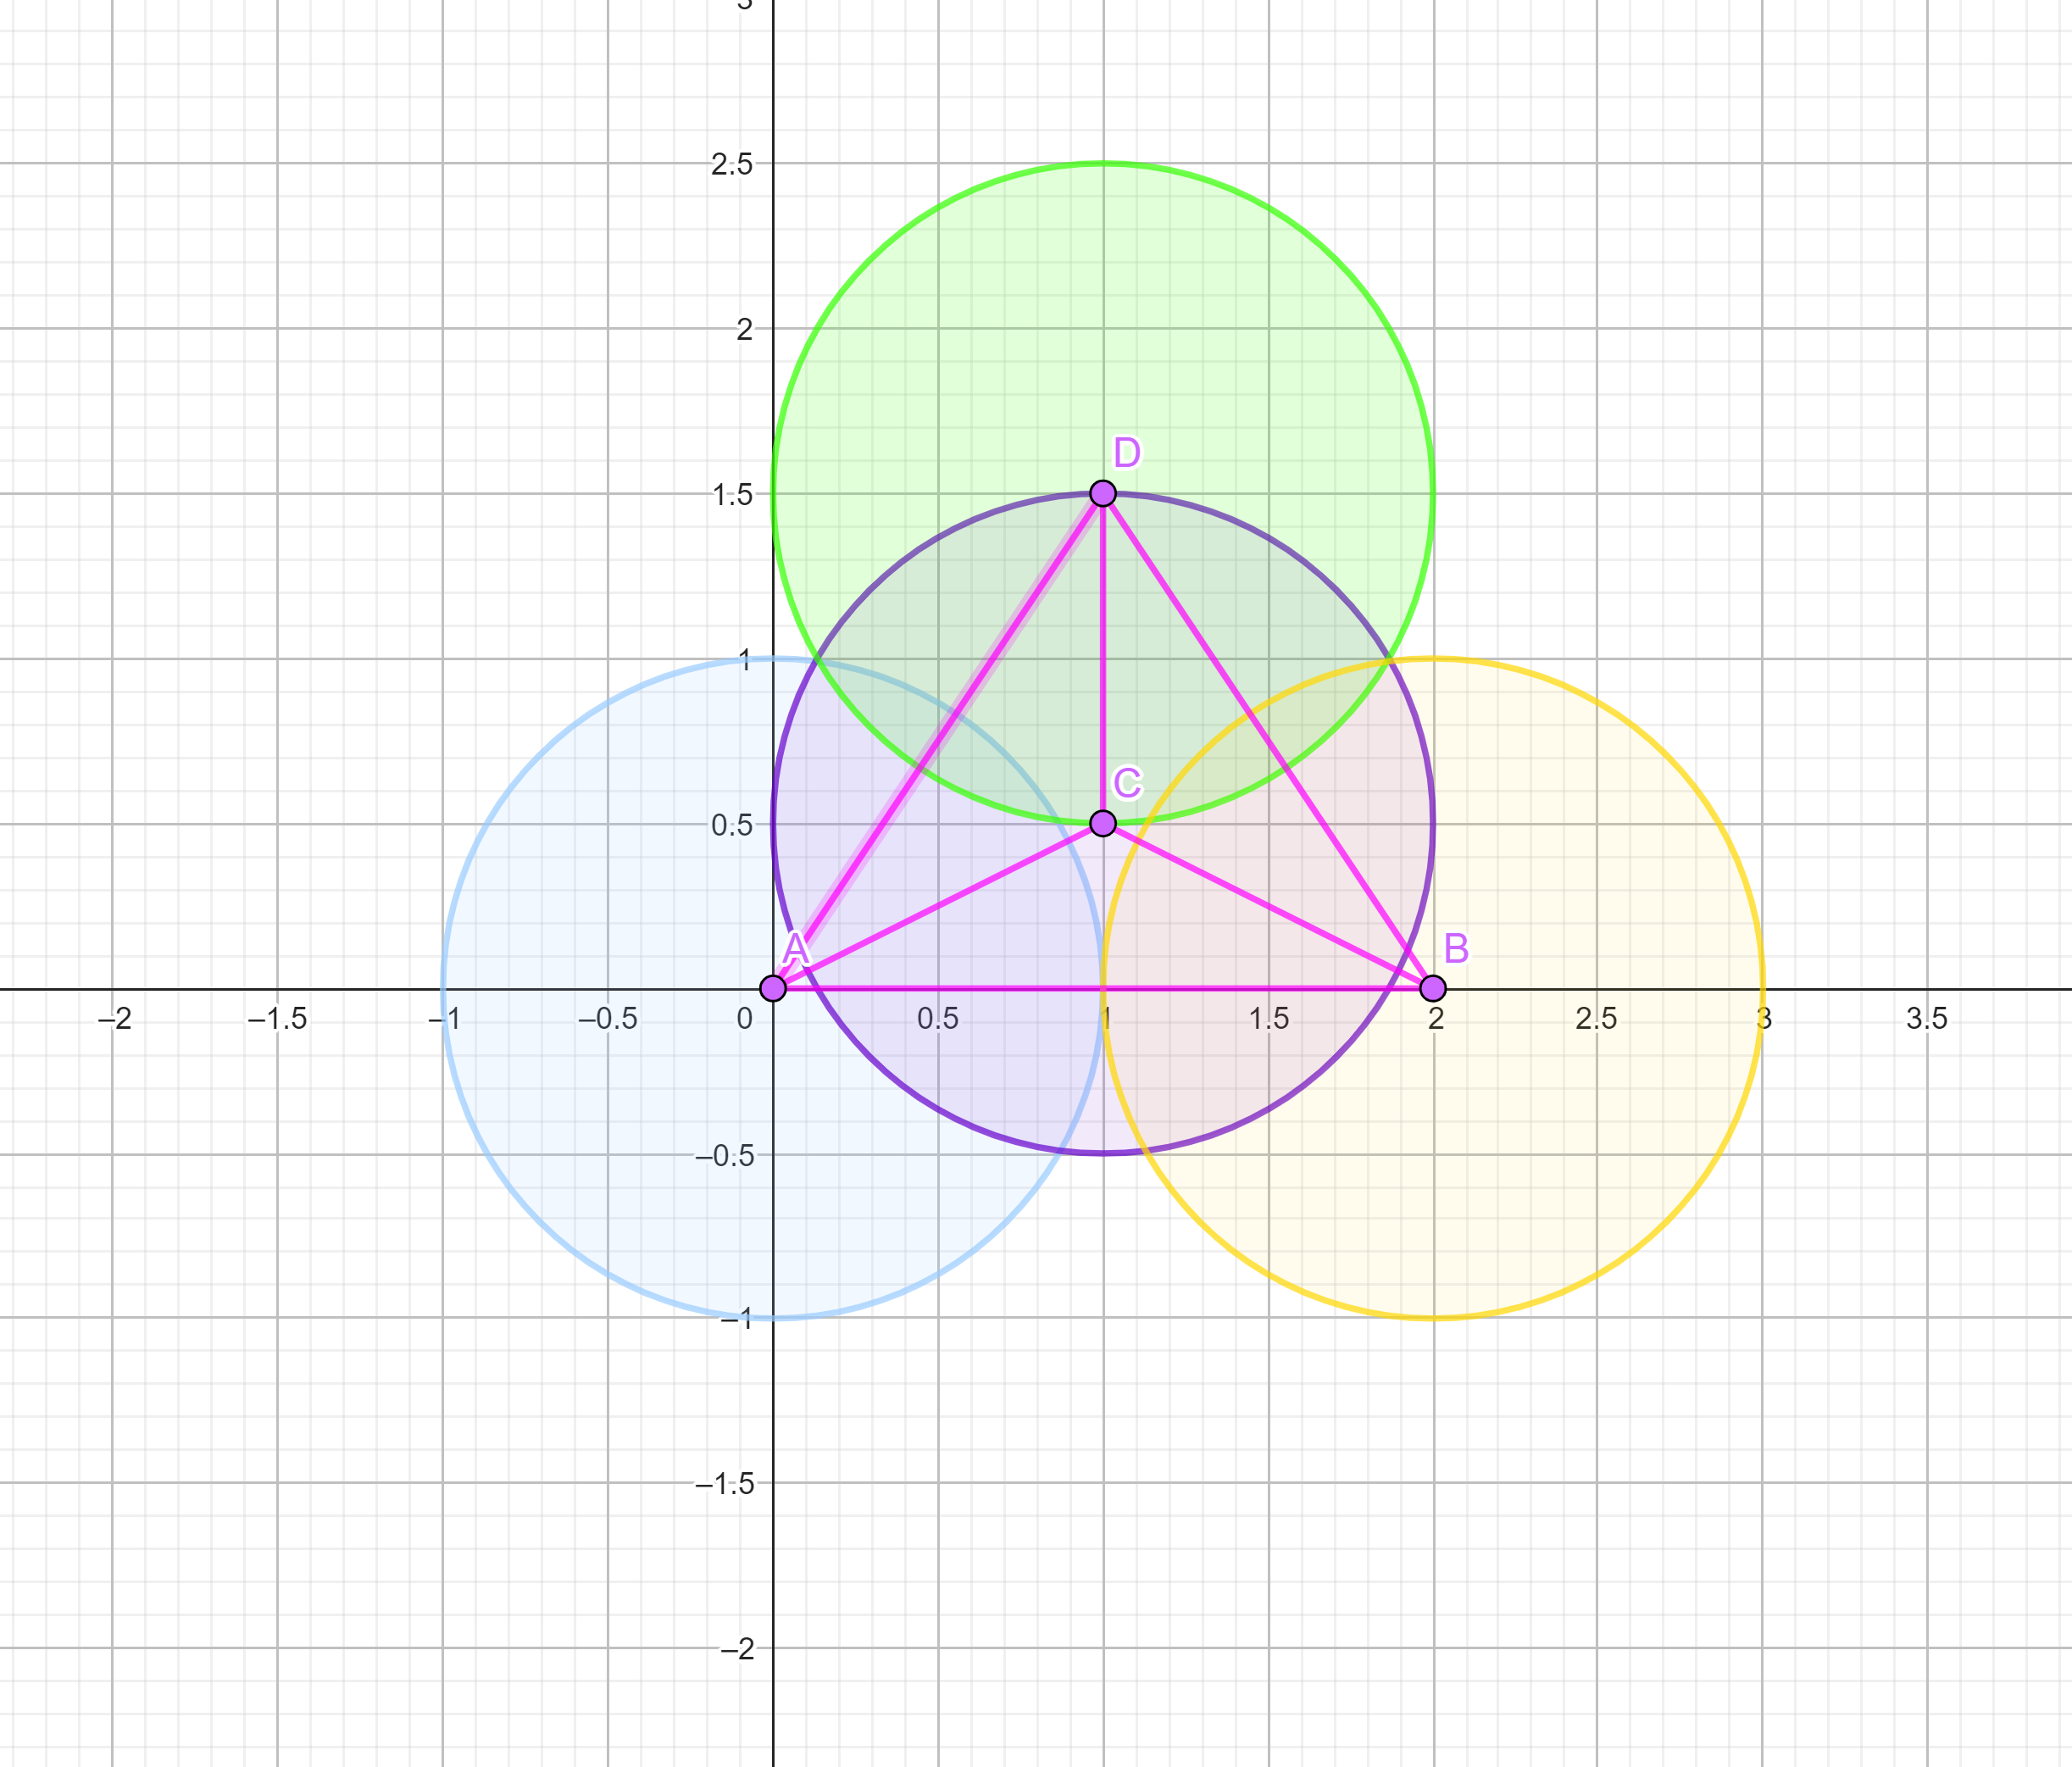
\includegraphics[scale=0.20] {graf4}
	  	\caption{\label{fig:1} Closed balls around the points and skeleton of $VR_{2}(S)$ . }
	  \end{figure}
	  
	
	 

	\subsection{Voronoi diagram} In this exercise I will find a configuration of $n \in \mathbb{N}, n \geq 3$ points in the plane such that their Voronoi diagram will have a cell with $n-1$ vertices. First let's construct convex $n-1$ polygon and put one point in its centre. Let's name the polygon $P$ and the point in the centre $O$. This is the first point in the plane. $P$ will be the cell with $n-1$ vertices that we are looking for. Let's treat vertices of $P$ as Vronoi vertices.  Now we have to configure remaining $n-1$ points. For every Voronoi vertex we draw a circle with the centre of origin in the mentioned Vornoi vertex and with radius which is the distance between mentioned Voronoi vertex and $O$. Two neighbouring circles intersect two times - first time in $O$ and second time where another point from the configuration is supposed to be. Those neighbouring intersections, together with $O$, is the configuration we are looking for. When we have  the configuration, we only have to draw the Voronoi diagram. Example for $n=8$ can be seen on Figure $4$ (configuration points are red, on example can also be seen circles which are not part of the Voronoi diagram but were used for constructiong the configuration points).
	
	\begin{figure}
		\centering
		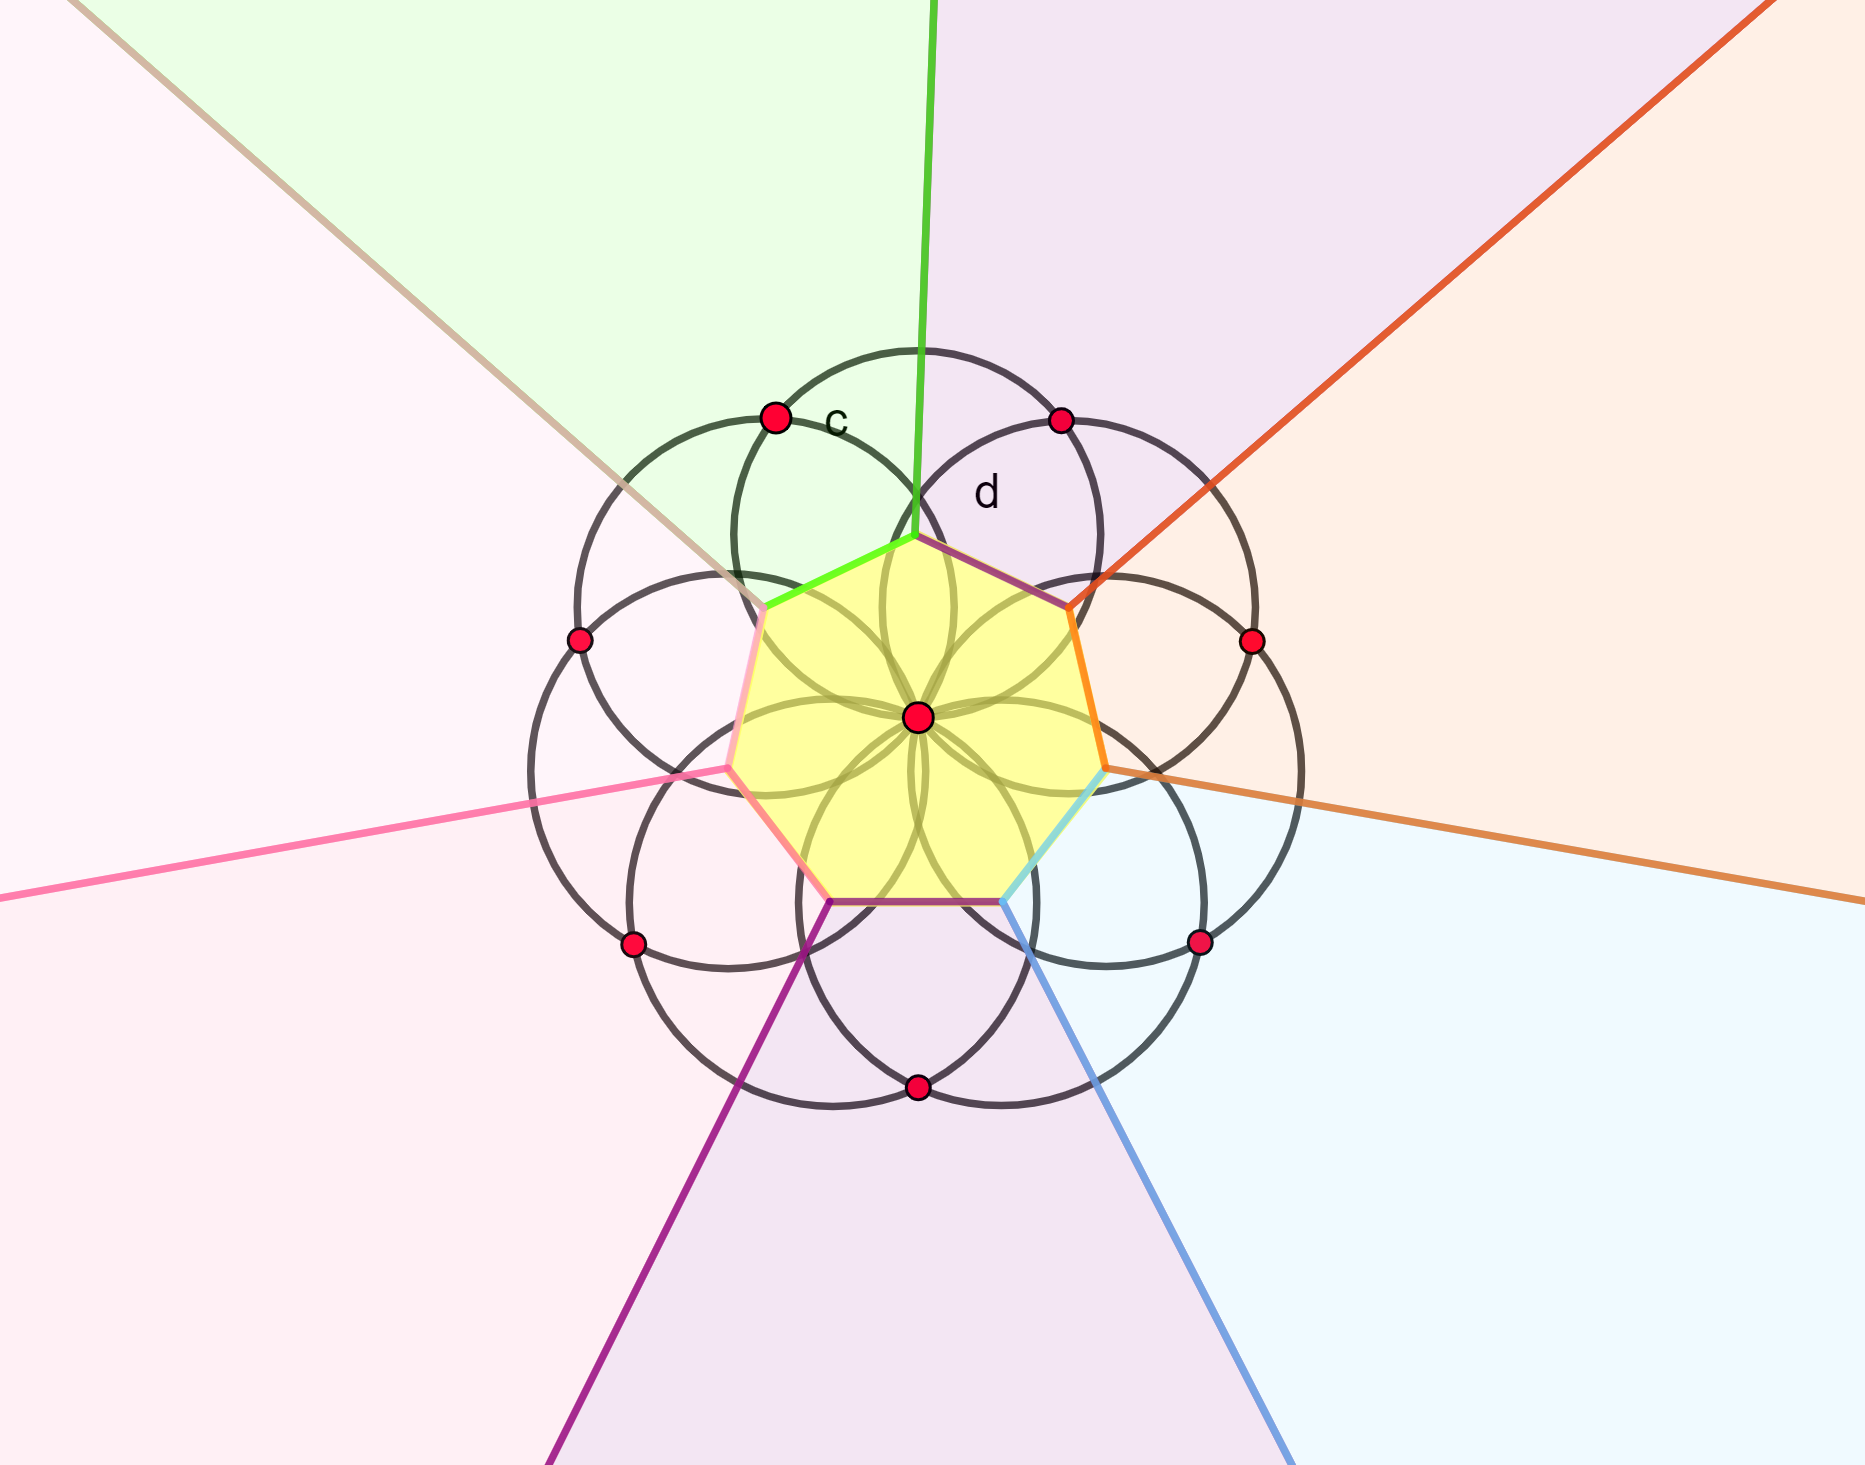
\includegraphics[scale=0.20] {graf2}
		\caption{\label{fig:4} Example for $n=8$ for Exercise 1.3 }
	\end{figure}

	\subsection{Chessboard Complex}
	\textbf{(a)} In this exercise I showed that the chessboard complex $\Delta_{3 \times 2}$ is homemorphic to the circle $S^1$ by showing that the simplicial complex I obtain is a $1$-dimansional connected manifold with no boundary.  \\
	
	I labelled chessboard cells with letters from $A$ to $F$ as can be seen on Figure 5. Consequently the simplicial complex $K$ I got was: 
	
	$$K = \{A,B,C,D,E,F,AD,AF,BC,BE,FC,DE\}$$
	
	Because the simplicial complex I got is a 1-dimensional (basically a graph) that means that link $Lk(v)$ of any vertex $v$ (0-dimensional simplex from our  simplicial complex $K$) is its neighbourhood. From the Figure 5 can be seen that every vertex has two neighbours (two zero dimensional simplices). That means that the neighbourhood of every vertex is homeomorphic to $S^0$ and consequently $K$ is $1$-dimensional manifold without boundary(from definition). From the Figure 5 can be seen that $K$ is also connected. \\
	
	\begin{figure}
		\centering
		\includegraphics[scale=0.20] {graf5}
		\caption{\label{fig:5}chessboard complex $\Delta_{3 \times 2}$ and the simplical complex it obtains. }
	\end{figure}
	
	
	\textbf{(b)}  In this exercise I showed that the chessboard complex $\Delta_{4 \times 3}$ is homemorphic to a torus $S^1 \times S^1$ by showing that the simplicial complex I obtain is a orientable $2$-dimensional connected manifold with no boundary with Euler characteristic 0.  \\
	
	The simplicial complex can be seen on Figure 6. Because the chessboard complex dimansions are $4 \times 3$ by using combinatorics I knew there will be $4 \cdot 3 \cdot 2 = 24$ 2-dimensional simplices. First I labelled chessboard cells with letters and decided to pick one random cell and fix it. Then I drew the body of all simplicial complexes which included the fixed point. From the drawing I saw that the link of the fixed point is 6-polygon, which is homeomorphic to $S^1$. Because I chose the fixed point randomly this stands for all points in simplical complex. That means that  that the simplicial complex I obtained is a orientable $2$-dimensional connected manifold with no boundary. The proof that simplicial complex is orienatable is seen on Figure 6. From the drawing of the simplicial complex I can also conclude that the Euler characteristic is: $\chi = 12 - 36 + 24= 0$ \\
	
	\begin{figure}
		\centering
		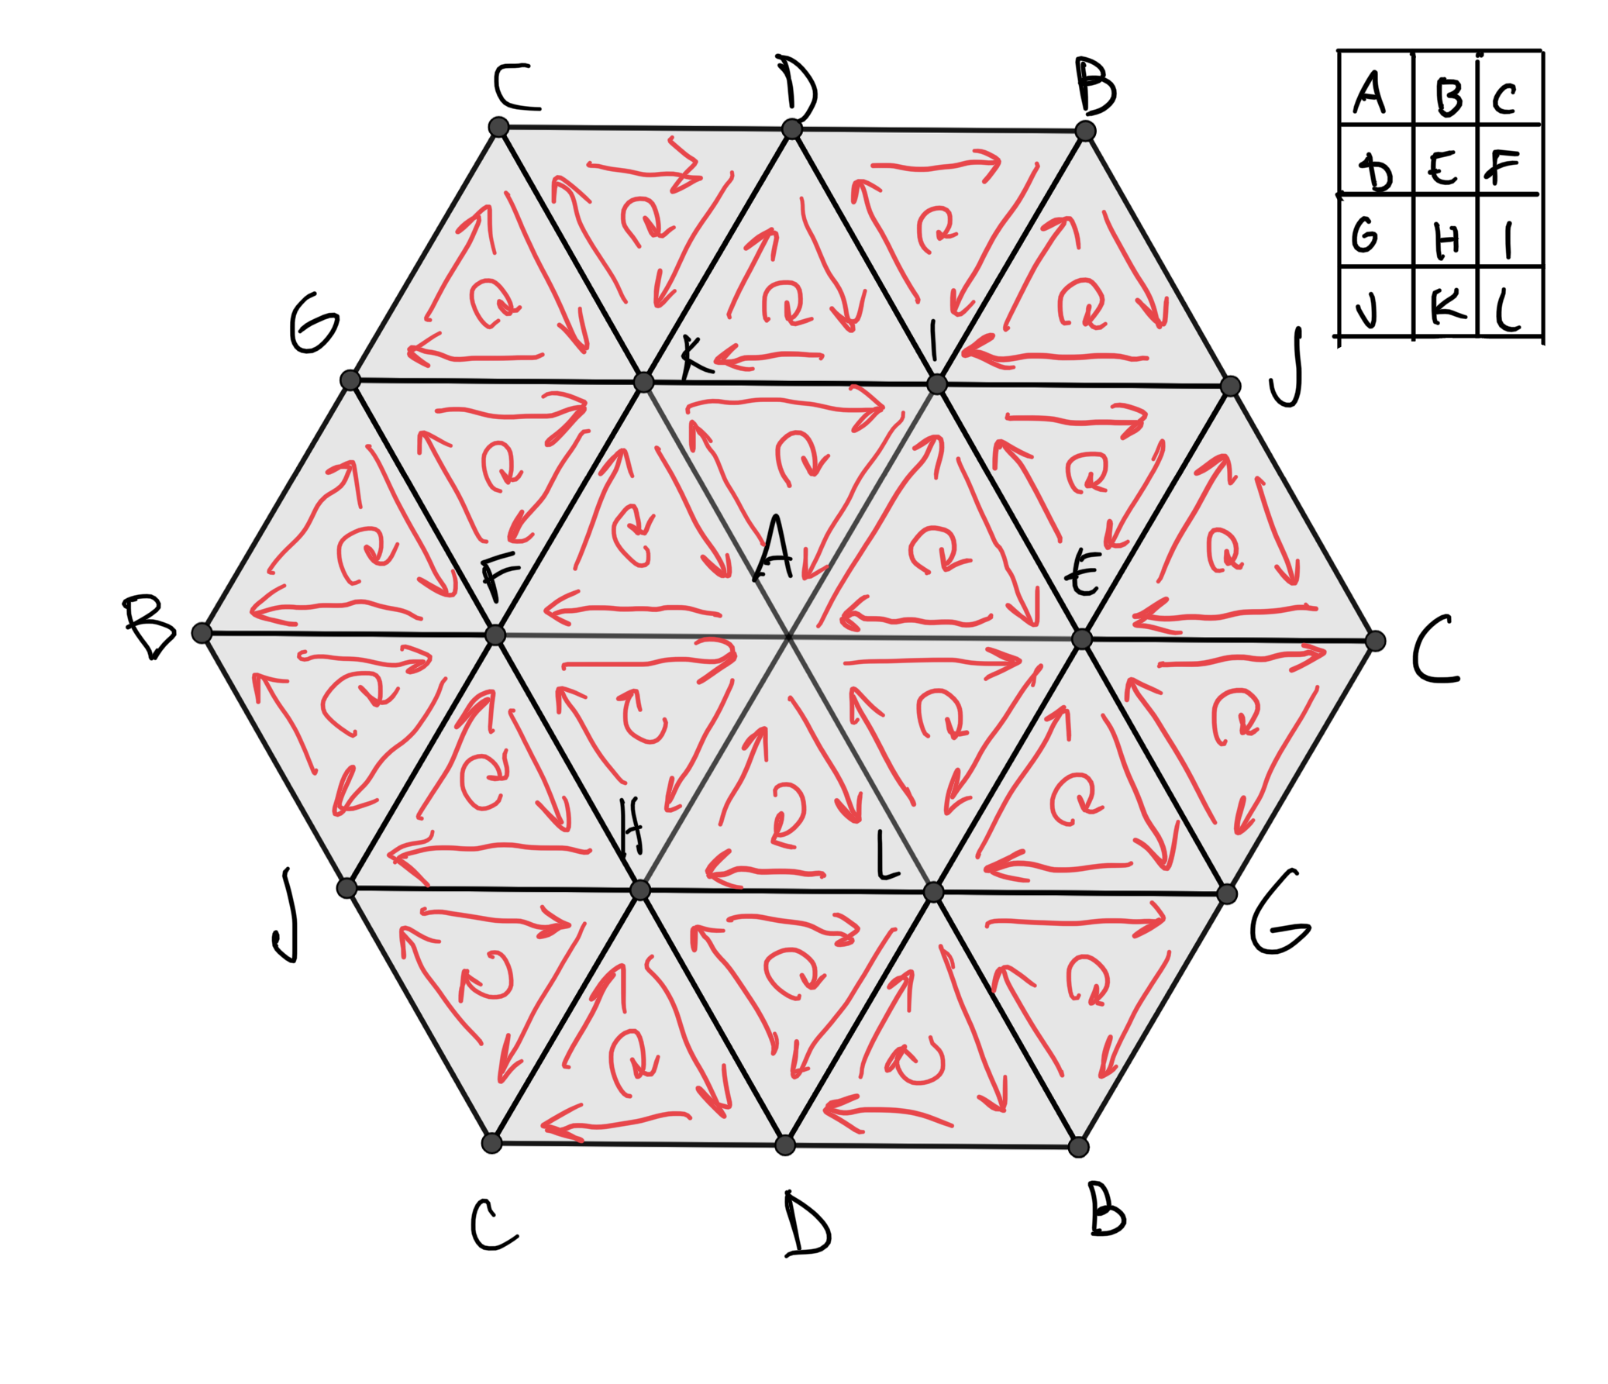
\includegraphics[scale=0.20] {graf6}
		\caption{\label{fig:6} Chessboard complex $\Delta_{4 \times 3}$ and the simplicial complex it obtains with its orientation. }
	\end{figure}
	
	\textbf{(c)} In the last exercise I showed that the chessboard complex $\Delta_{n \times (n-1)}$ is a manifold for all $n$. I showed that the simplicial complex I obtained is a $(n-2)$-dimensional manifold. \\
	
	Let $v$ be a random point in beforementioned simplicial complex. We want to see what its link is. $v$ is a part of $(n-1)!$ simplices, each with dimension $(n-2)$. We want to prove that $link(v)$ is homeomorphic to $S^{(n-3)}$. Each of the $(n-1)!$ simplices is connected with other simplices. Two neighbouring simplices are sharing the same face. That is possible, because there are $n$ rows in chessboard complex - that means one row is always empty so we can always find a simplex that is connected to other simplex by its face, we just have to change one of the rows with the empty one. In other words, simplies that share face (their intersection is their face) differ only by one point and that point can be found in the same column, just different row. Consequently simplices are connected with their faces which means $link(v)$ is also connected with its faces (so there are no holes). Also, $link(v)$ has one dimension less than simplices that contains $v$ so its dimension is $(n-3)$. That means $link(v)$ is homeomorphic to $S^{(n-3)}$.
	
	
	\section{Programming problems}
	
	\subsection{Line sweep triangulation}
	\begin{figure}
		\centering
		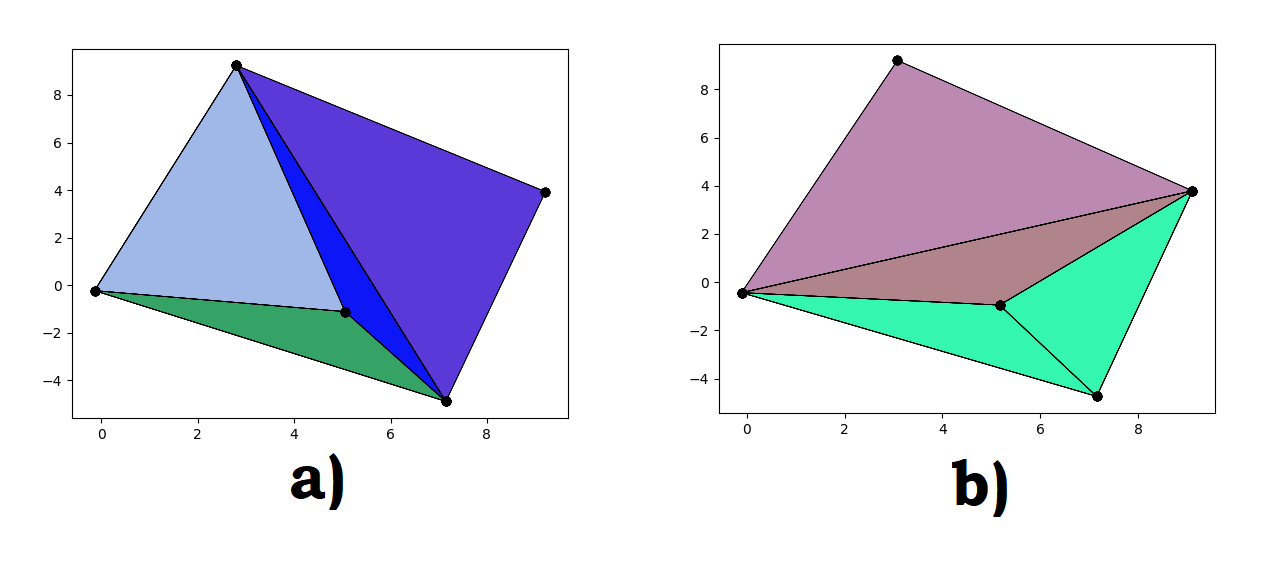
\includegraphics[scale=0.5] {graf7}
		\caption{\label{fig:7} Line sweep trinagulation for S = [(0, 0), (3, 9), (5, -1), (9, 4), (7, -5)], a)  triangulation(S, vertical = True), b) triangulation(S, vertical = False) }
	\end{figure}
	
	\begin{figure}
		\centering
		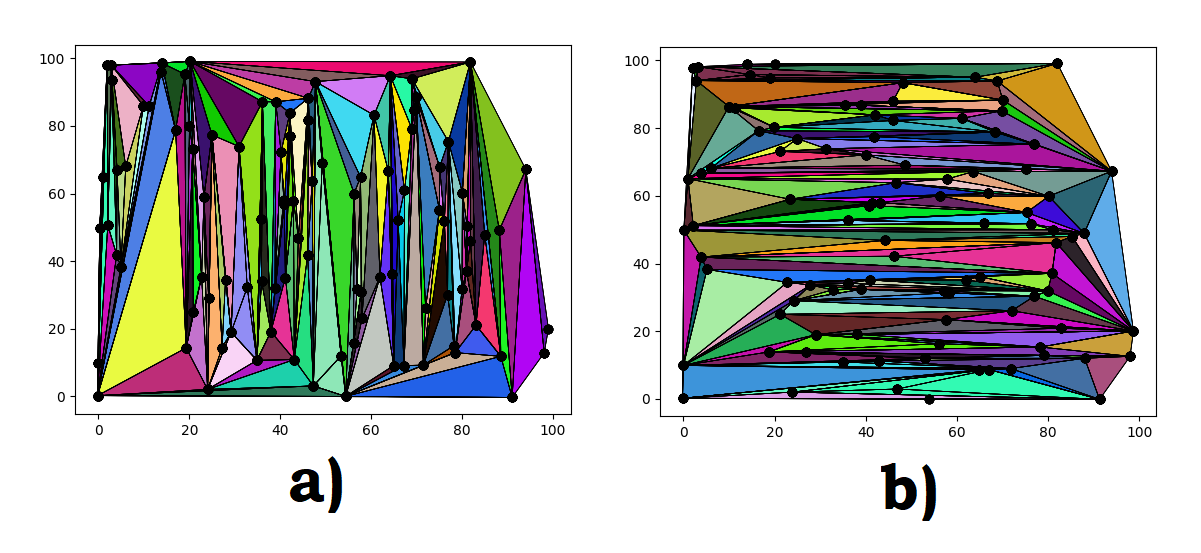
\includegraphics[scale=0.5] {graf8}
		\caption{\label{fig:8} Line sweep trinagulation where S is a set of random 100 points, a)  triangulation(S, vertical = True), b) triangulation(S, vertical = False) }
	\end{figure}
	
	\begin{figure}
		\centering
		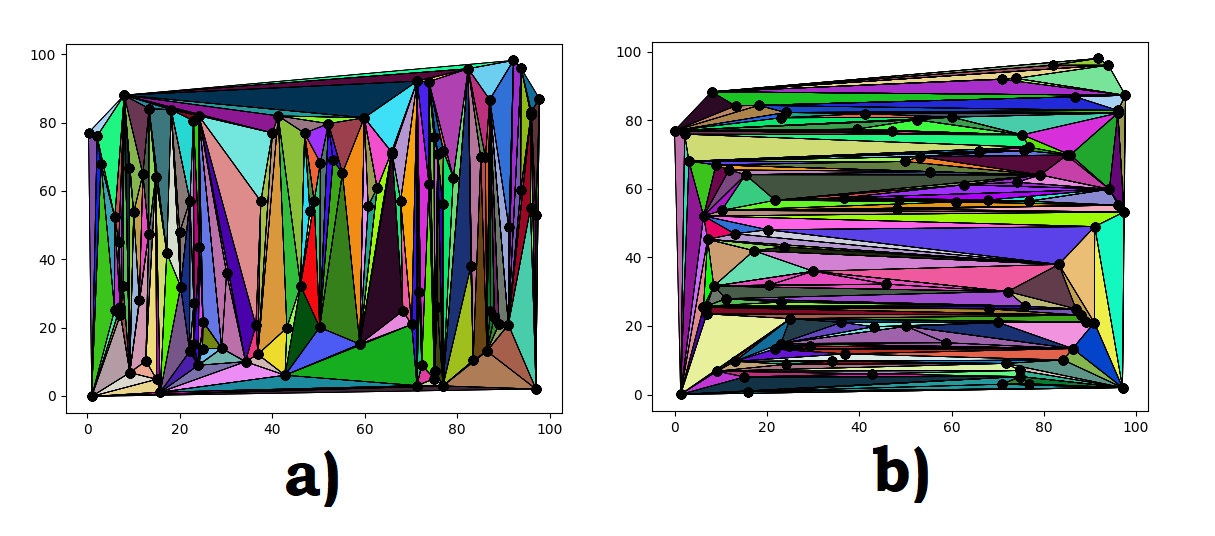
\includegraphics[scale=0.5] {graf9}
		\caption{\label{fig:9} Line sweep trinagulation where S is a set of random 100 points, a)  triangulation(S, vertical = True), b) triangulation(S, vertical = False) }
	\end{figure}
	My file linesweeptriangulation.py contains a function triangulate(S, vertical=True), which returns a list of edges and a list of triangles which is a line sweep trinagulation. Triangulation line can be vertical which is by default or horizontal if second parameter is False. Function triangulate(S, vertical = True) also draws the triangulation. My file alsod contains function generify(S) which adds a little noise to the points. On Figure 7 can be seen example with sample input S = [(0, 0), (3, 9), (5, -1), (9, 4), (7, -5)] with both resulting triangulations - one for vertical = True and one for vertical = False.
	
	I also made up two more test cases, both of which consist of 100 points. Resulting triangulations can be seen on Figures 8 and 9, on left sides resulting triangulations for vertical = True and on the right side for vertical = False.
	
	\subsection{Delauney triangulation}
	My file delauney.py contains function optimize(T), which takes triangulation T and outputs Delauney's triangulation. It also drew three drawings, two are of a trinagulation T and last one is Delauney triangulation. I tested in on many cases with 100+ points, two of the cases can be seen on Figures 10 and 11. I used Delaunay's angle condition.
	
	\begin{figure}
		\centering
		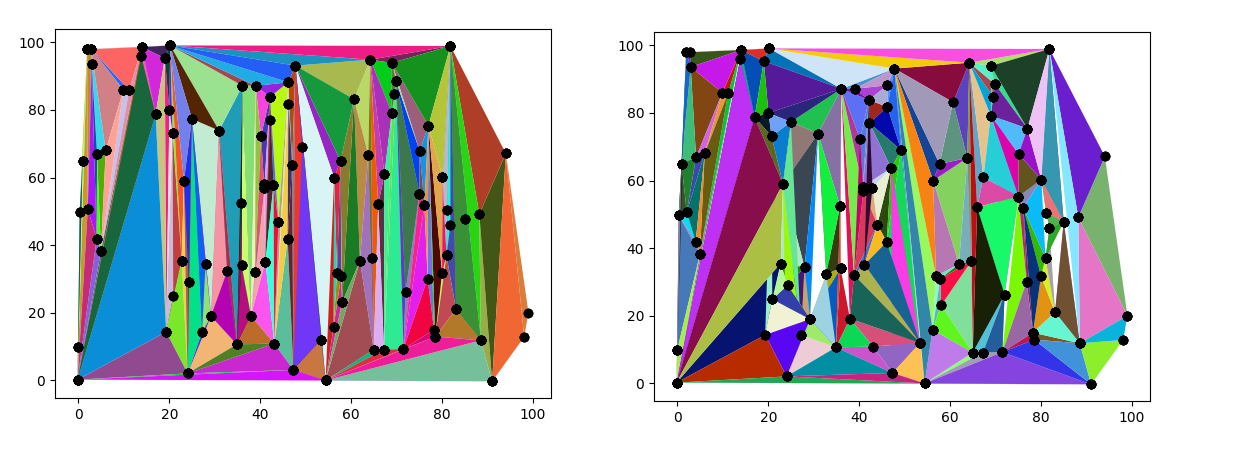
\includegraphics[scale=0.5] {graf10}
		\caption{\label{fig:10} left: regular trinagulation right: Delauney triangulation}
	\end{figure}
	
	\begin{figure}
		\centering
		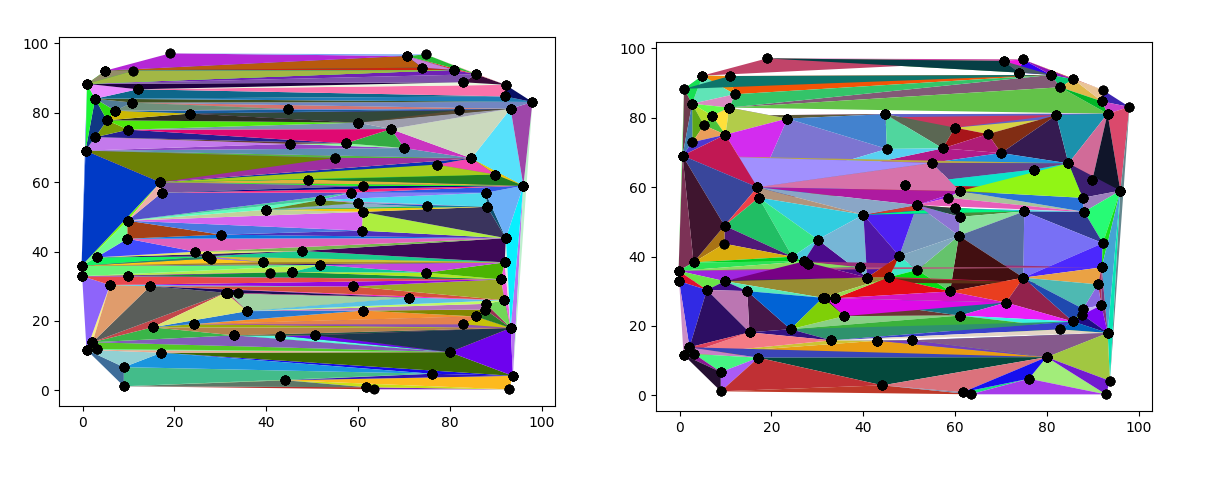
\includegraphics[scale=0.5] {graf11}
		\caption{\label{fig:11} left: regular trinagulation right: Delauney triangulation }
	\end{figure}
	 
	\subsection{Orientation of surfaces}
	My file orientable.py contains a function orientableQ(T), which returns True if
	a 2-manifold given by its triangulation T is orientable and False otherwise. It also includes a function orientable(T), which returns the list of oriented triangles if the 2-manifold is orientable and None otherwise. \\
	
	I will describe how my function works by listing all the important steps: 
	
	\begin{enumerate}
		\item Create two empty lists, one for already oriented triangles and other to have the same  functionality as stack, which consists of triangles whose neighbours have to be oriented. The first item in both lists is first triangle from triangulation T.
		\item While list stack is not empty pop a triangle from it and orient its neighbours. If its neighbours are already oriented check if the new orientation agrees with the old one. If not return False. 
		\item If its neighbours are not oriented, orient them and put them on stack.
	\end{enumerate}

I tested my function on two cases from homework instructions and on triangulations of a torus, a Klein bottle, a sphere, a cylinder and a Moebius band. I mostly used the triangulations I found in Introduction to Persistent Homology by Žiga Virk. Some of them I also found on the internet. Results of the test are written below but they can also be found in my file.  \\

Torus \\
\noindent $torus = [(1,2,5),(2,5,6),(2,3,6),(1,3,7),(3,6,7),(5,7,1),(5,4,6),(4,6,8),(6,7,8),(7,8,9), $\\
$(7,5,9),(5,4,9),(1,4,8),(8,1,2),(2,8,9),(9,2,3),(4,9,3),(4,3,1)] $ \\
$orientableQ(torus) = True $ \\
$orientable(torus) = [(1, 2, 5), (2, 6, 5), (1, 5, 7), (1, 8, 2), (1, 4, 8), 
 (2, 8, 9), (7, 9, 8), (2, 9, 3), 
  \\(2, 3, 6), (3, 9, 4), (4, 9, 5),  (1, 3, 4), 
  (1, 7, 3), (3, 7, 6), (6, 7, 8), (4, 6, 8), (4, 5, 6), (5, 9, 7)]$ \\
  
  Klein bottle \\
  \noindent $kleinbottle = [(1,2,4),(2,4,6),(2,3,6),(1,3,7),(3,6,7),(5,7,1),(5,4,6),(5,6,8),(6,7,8),(7,8,9),
  \\ (7,5,9),(5,4,9),(1,5,8),(8,1,2),(2,8,9),(9,2,3),(4,9,3),(4,3,1)] $\\
  $orientableQ(kleinbottle) = False $ \\
  $orientable(kleinbottle) = None $\\
  
  Sphere \\
 \noindent $sphere = [(1, 2, 4), (1,2,3),(3,2,4),(1,3,4)] $\\
 $orientableQ(sphere) = True $ \\
 $orientable(sphere) = [(1, 2, 4), (1, 3, 2), (2, 3, 4), (1, 4, 3)] $\\
 
   Cylinder \\
 \noindent $cylinder = [(1,4,6),(1,6,2),(2,5,6),(2,3,5),(3,4,5),(1,3,4)] $\\
 $orientableQ(cylinder) = True $ \\
 $orientable(cylinder) = [(1, 4, 6), (1, 6, 2), (1, 3, 4), (3, 5, 4), (2, 5, 3), (2, 6, 5)] $\\
 
   Moebius band \\
 \noindent $moebiusband = [(1,2,4),(1,3,4),(3,4,6),(3,5,6),(5,6,8),(5,7,8),(7,8,1),(1,2,7)] $\\
 $orientableQ(moebiusband) = False $ \\
 $orientable(moebiusband) = None $\\
  
  
  





	
	
	
	
	
	
	
	
	

	
	% --------------------------------------------------------------
	%     You don't have to mess with anything below this line.
	% --------------------------------------------------------------
	
	
\end{document}    